\subsubsection{Example}

    \begin{itemize}[noitemsep,topsep=0pt]
      \item Starting position: (-1.0, -8.0, 34.0)
      \item End position: (-4.0, 1.0, 8.0) 
      \item Euclidean distance from the object: 9.0
      \item Object can be seen: True
      \item Success: True
      \item Object type: a large trash pile
      
    \end{itemize}
    

    \begin{center}
    \includegraphics[width=0.7\linewidth]{images/Sonnet-CityNew/24_r0_.pdf}
    \end{center}
    

    \begin{center}
    \includegraphics[width=0.7\linewidth]{images/Sonnet-CityNew/24_r0__sit_awareness.pdf}
    \end{center}
    

    \begin{drama}
    \Character{Benchmark}{re}
    \Character{Claude 3.5 Sonnet}{gpt}
    
\respeaks: \( < \)Context\( > \)
    You are in command of a UAV, tasked with finding a large trash pile.
\( < \)/Context\( > \) \texttt{(REST OF THE PROMPT)}
\respeaks: Image 1:
\StageDir{\re{} presents \gpt{} with a relevant image}

    \begin{center}
    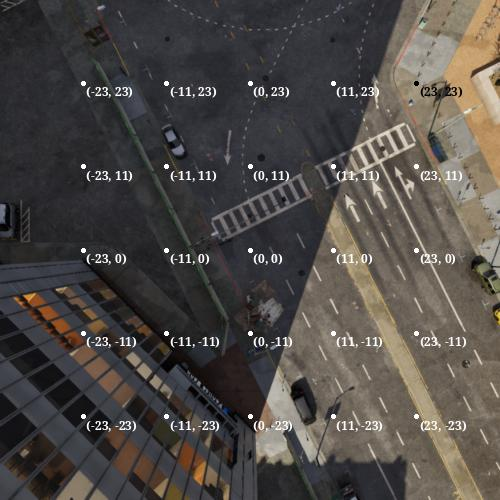
\includegraphics[width=0.5\linewidth]{images/Sonnet-CityNew/24_r0__0.jpg}
    \end{center}
    
\respeaks: Your current altitude is 34 meters above ground level.
\gptspeaks: \( < \)Reasoning\( > \)I need to systematically search the area for a large trash pile. From my current altitude of 34 meters, I can see a good portion of the area, but I need to get lower to better identify objects. I'll start by moving towards the center-right area (11, 0) and descending to get a better view, as this area seems to have some potential objects that need closer inspection.\( < \)/Reasoning\( > \)
\( < \)Action\( > \)(11, 0, -20)\( < \)/Action\( > \)
\respeaks: Image 2:
\StageDir{\re{} presents \gpt{} with a relevant image}

    \begin{center}
    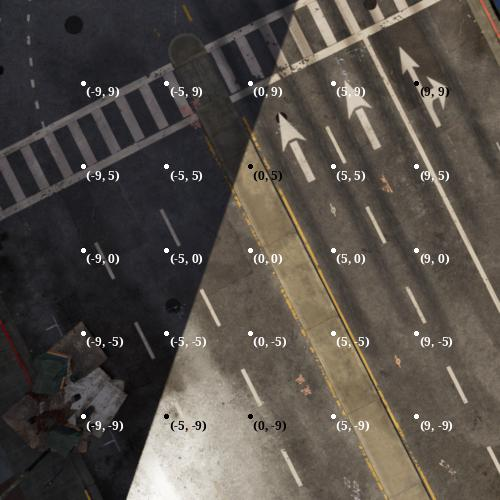
\includegraphics[width=0.5\linewidth]{images/Sonnet-CityNew/24_r0__1.jpg}
    \end{center}
    
\respeaks: Your current altitude is 14 meters above ground level.
\gptspeaks: \( < \)Reasoning\( > \)I can see what appears to be some debris or potential trash in the lower left corner of the image around coordinates (-9, -9). I'll move towards that location while maintaining my current low altitude to get a better look at what appears to be the target.\( < \)/Reasoning\( > \)
\( < \)Action\( > \)(-9, -9, 0)\( < \)/Action\( > \)
\respeaks: Image 3:
\StageDir{\re{} presents \gpt{} with a relevant image}

    \begin{center}
    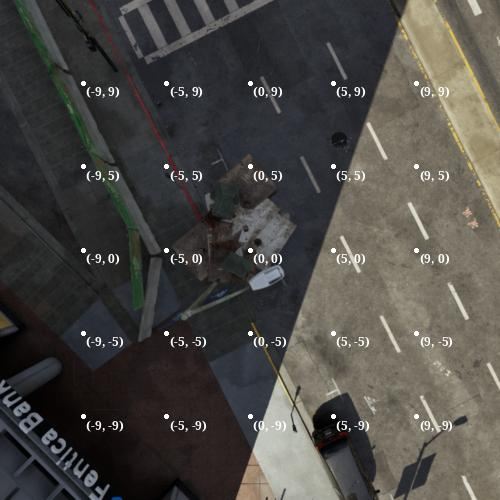
\includegraphics[width=0.5\linewidth]{images/Sonnet-CityNew/24_r0__2.jpg}
    \end{center}
    
\respeaks: Your current altitude is 14 meters above ground level.
\gptspeaks: \( < \)Reasoning\( > \)I can now clearly see a pile of debris/trash in my field of view, but I need to get a bit lower to ensure I'm within 10 meters of it as required by the objective. The pile appears to be centered around (-5, 0). I'll move slightly to better center on it and descend to about 8 meters altitude to ensure I'm meeting the requirement of being below 10 meters.\( < \)/Reasoning\( > \)
\( < \)Action\( > \)(-5, 0, -6)\( < \)/Action\( > \)
\respeaks: Image 4:
\StageDir{\re{} presents \gpt{} with a relevant image}

    \begin{center}
    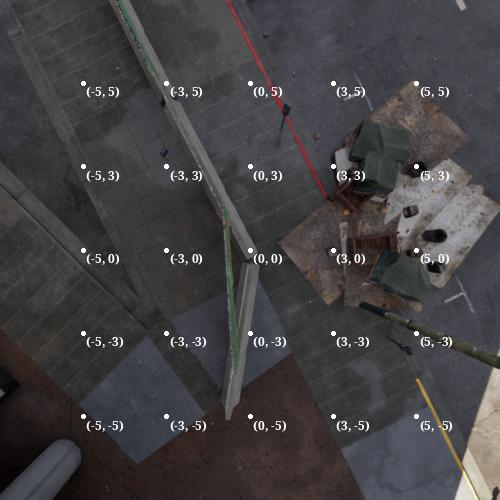
\includegraphics[width=0.5\linewidth]{images/Sonnet-CityNew/24_r0__3.jpg}
    \end{center}
    
\respeaks: Your current altitude is 8 meters above ground level.
\gptspeaks: \( < \)Reasoning\( > \)I can now clearly see the trash pile in my field of view, and I am positioned at 8 meters altitude, which is below the required 10 meters. The object is centered in my view, and I am at an appropriate height to confirm this is indeed the target.\( < \)/Reasoning\( > \)
FOUND
\end{drama}
\subsubsection{Example}

    \begin{itemize}[noitemsep,topsep=0pt]
      \item Starting position: (3.0, -17.0, 60.0)
      \item End position: (0.0, 0.0, 8.0) 
      \item Euclidean distance from the object: 8.0
      \item Object can be seen: True
      \item Success: True
      \item Object type: a fire
      
    \end{itemize}
    

    \begin{center}
    \includegraphics[width=0.7\linewidth]{images/Sonnet-CityNew/27_r0_.pdf}
    \end{center}
    

    \begin{center}
    \includegraphics[width=0.7\linewidth]{images/Sonnet-CityNew/27_r0__sit_awareness.pdf}
    \end{center}
    

    \begin{drama}
    \Character{Benchmark}{re}
    \Character{Claude 3.5 Sonnet}{gpt}
    
\respeaks: \( < \)Context\( > \)
    You are in command of a UAV, tasked with finding a fire.
\( < \)/Context\( > \) \texttt{(REST OF THE PROMPT)}
\respeaks: Image 1:
\StageDir{\re{} presents \gpt{} with a relevant image}

    \begin{center}
    
\includegraphics[width=0.5\linewidth]{images/Sonnet-CityNew/27_r0__0.jpg}
    \end{center}
    
\respeaks: Your current altitude is 60 meters above ground level.
\gptspeaks: \( < \)Reasoning\( > \)
I can see this is an urban environment viewed from above. Since I'm looking for a fire and need to search carefully, I should start by scanning the area systematically. I notice some open areas in the center of the image. I'll move to a central position and lower my altitude to get a better view of potential fire signs.
\( < \)/Reasoning\( > \)
\( < \)Action\( > \)(0, 0, -30)\( < \)/Action\( > \)
\respeaks: Image 2:
\StageDir{\re{} presents \gpt{} with a relevant image}

    \begin{center}
    
\includegraphics[width=0.5\linewidth]{images/Sonnet-CityNew/27_r0__1.jpg}
    \end{center}
    
\respeaks: Your current altitude is 30 meters above ground level.
\gptspeaks: \( < \)Reasoning\( > \)
From this lower altitude, I can see better details of the street. I notice what appears to be a small red glow or potential fire near the coordinates (0, -20). I should move closer to that location and lower my altitude further to confirm if this is the fire we're looking for.
\( < \)/Reasoning\( > \)
\( < \)Action\( > \)(0, -20, -20)\( < \)/Action\( > \)
\respeaks: Image 3:
\StageDir{\re{} presents \gpt{} with a relevant image}

    \begin{center}
    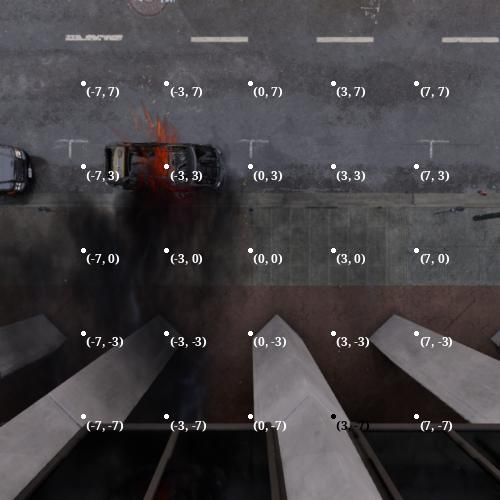
\includegraphics[width=0.5\linewidth]{images/Sonnet-CityNew/27_r0__2.jpg}
    \end{center}
    
\respeaks: Your current altitude is 10 meters above ground level.
\gptspeaks: \( < \)Reasoning\( > \)
I can now clearly see a car on fire near coordinates (-3, 3). I need to position myself directly above it at a height less than 10 meters to meet the objective requirements. I'll move to those coordinates and lower my altitude slightly to ensure I'm below 10 meters.
\( < \)/Reasoning\( > \)
\( < \)Action\( > \)(-3, 3, -2)\( < \)/Action\( > \)
\respeaks: Image 4:
\StageDir{\re{} presents \gpt{} with a relevant image}

    \begin{center}
    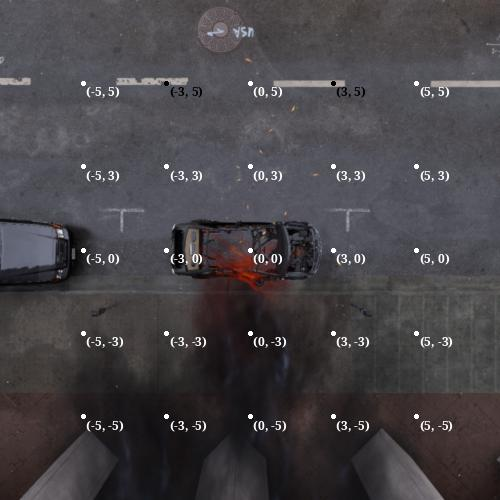
\includegraphics[width=0.5\linewidth]{images/Sonnet-CityNew/27_r0__3.jpg}
    \end{center}
    
\respeaks: Your current altitude is 8 meters above ground level.
\gptspeaks: \( < \)Reasoning\( > \)
I am now positioned at 8 meters above the burning car, which is clearly visible in my field of view at the center of the image. This meets all the requirements: the fire is in view, I am centered above it, and my altitude is below 10 meters (specifically at 8 meters).
\( < \)/Reasoning\( > \)
FOUND
\end{drama}
